\chapter{Combinatorics}

\index{combinatorics}

\key{Combinatorics} studies methods for counting
combinations of objects.
Usually, the goal is to find a way to
count the combinations efficiently
without generating each combination separately.

As an example, let's consider a problem where
our task is to calculate the number of representations
for an integer $n$ as a sum of positive integers.
For example, there are 8 representations
for the number $4$:
\begin{multicols}{2}
\begin{itemize}
\item $1+1+1+1$
\item $1+1+2$
\item $1+2+1$
\item $2+1+1$
\item $2+2$
\item $3+1$
\item $1+3$
\item $4$
\end{itemize}
\end{multicols}

A combinatorial problem can often be solved
using a recursive function.
In this case, we can define a function $f(n)$
that counts the number of representations for $n$.
For example, $f(4)=8$ according to the above example.
The function can be recursively calculated as follows:
\begin{equation*}
    f(n) = \begin{cases}
               1               & n = 1\\
               f(1)+f(2)+\ldots+f(n-1)+1 & n > 1\\
           \end{cases}
\end{equation*}
The base case is $f(1)=1$,
because there is only one way to represent the number 1.
Otherwise, we go through all possibilities for
the last number in the sum.
For example, in when $n=4$, the sum can end
with $+1$, $+2$ or $+3$.
In addition, we also count the representation
that only contains $n$.

The first values for the function are:
\[
\begin{array}{lcl}
f(1) & = & 1 \\
f(2) & = & 2 \\
f(3) & = & 4 \\
f(4) & = & 8 \\
f(5) & = & 16 \\
\end{array}
\]
It turns out that the function also has a closed-form formula
\[
f(n)=2^{n-1},
\]
which is based on the fact that there are $n-1$
possible positions for +-signs in the sum,
and we can choose any subset of them.

\section{Binomial coefficient}

\index{binomial coefficient}

A \key{binomial coefficient} ${n \choose k}$
is the number of ways we can choose a subset
of $k$ elements from a set of $n$ elements.
For example, ${5 \choose 3}=10$,
because the set $\{1,2,3,4,5\}$
has 10 subsets of 3 elements:
\[ \{1,2,3\}, \{1,2,4\}, \{1,2,5\}, \{1,3,4\}, \{1,3,5\}, 
\{1,4,5\}, \{2,3,4\}, \{2,3,5\}, \{2,4,5\}, \{3,4,5\} \]

\subsubsection{Formula 1}

Binomial coefficients can be
recursively calculated as follows:

\[
{n \choose k}  =  {n-1 \choose k-1} + {n-1 \choose k}
\]

The idea is to consider a fixed
element $x$ in the set.
If $x$ is included in the subset,
the remaining task is to choose $k-1$
elements from $n-1$ elements,
and otherwise
the remaining task is to choose $k$ elements from $n-1$ elements.

The base cases for the recursion are as follows:
\[
{n \choose 0}  =  {n \choose n} = 1
\]

The reason for this is that there is always
one way to construct an empty subset,
or a subset that contains all the elements.

\subsubsection{Formula 2}

Another way to calculate binomial coefficients is as follows:
\[
{n \choose k}  =  \frac{n!}{k!(n-k)!}.
\]

There are $n!$ permutations for $n$ elements.
We go through all permutations and in each case
select the first $k$ elements of the permutation
to the subset.
Since the order of the elements in the subset
and outside the subset doesn't matter,
the result is divided by $k!$ and $(n-k)!$

\subsubsection{Properties}

For binomial coefficients,
\[
{n \choose k}  =  {n \choose n-k},
\]
because we can either select $k$
elements to the subset,
or select $n-k$ elements that
will be outside the subset.

The sum of binomial coefficients is
\[
{n \choose 0}+{n \choose 1}+{n \choose 2}+\ldots+{n \choose n}=2^n.
\]

The reason for the name ''binomial coefficient''
is that

\[ (a+b)^n =
{n \choose 0} a^n b^0 + 
{n \choose 1} a^{n-1} b^1 +
\ldots + 
{n \choose n-1} a^1 b^{n-1} +
{n \choose n} a^0 b^n. \]

\index{Pascal's triangle}

Binomial coefficients also appear in
\key{Pascal's triangle}
whose border consists of 1's,
and each value is the sum of two
above values:
\begin{center}
\begin{tikzpicture}{0.9}
\node at (0,0) {1};
\node at (-0.5,-0.5) {1};
\node at (0.5,-0.5) {1};
\node at (-1,-1) {1};
\node at (0,-1) {2};
\node at (1,-1) {1};
\node at (-1.5,-1.5) {1};
\node at (-0.5,-1.5) {3};
\node at (0.5,-1.5) {3};
\node at (1.5,-1.5) {1};
\node at (-2,-2) {1};
\node at (-1,-2) {4};
\node at (0,-2) {6};
\node at (1,-2) {4};
\node at (2,-2) {1};
\node at (-2,-2.5) {$\ldots$};
\node at (-1,-2.5) {$\ldots$};
\node at (0,-2.5) {$\ldots$};
\node at (1,-2.5) {$\ldots$};
\node at (2,-2.5) {$\ldots$};
\end{tikzpicture}
\end{center}

\subsubsection{Boxes and balls}

''Boxes and models'' is a useful model,
where we count the ways to
place $k$ balls in $n$ boxes.
Let's consider three cases:

\textit{Case 1}: Each box can contain
at most one ball.
For example, when $n=5$ and $k=2$,
there are 10 solutions:

\begin{center}
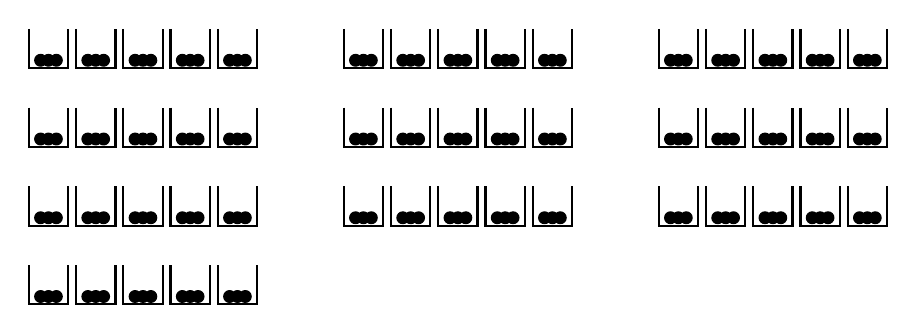
\begin{tikzpicture}[scale=0.5]
\newcommand\lax[3]{
\path[draw,thick,-] (#1-0.5,#2+0.5) -- (#1-0.5,#2-0.5) --
                    (#1+0.5,#2-0.5) -- (#1+0.5,#2+0.5);
\ifthenelse{\equal{#3}{1}}{\draw[fill=black] (#1,#2-0.3) circle (0.15);}{}
\ifthenelse{\equal{#3}{2}}{\draw[fill=black] (#1-0.2,#2-0.3) circle (0.15);}{}
\ifthenelse{\equal{#3}{2}}{\draw[fill=black] (#1+0.2,#2-0.3) circle (0.15);}{}
}
\newcommand\laa[7]{
    \lax{#1}{#2}{#3}
    \lax{#1+1.2}{#2}{#4}
    \lax{#1+2.4}{#2}{#5}
    \lax{#1+3.6}{#2}{#6}
    \lax{#1+4.8}{#2}{#7}
}

\laa{0}{0}{1}{1}{0}{0}{0}
\laa{0}{-2}{1}{0}{1}{0}{0}
\laa{0}{-4}{1}{0}{0}{1}{0}
\laa{0}{-6}{1}{0}{0}{0}{1}
\laa{8}{0}{0}{1}{1}{0}{0}
\laa{8}{-2}{0}{1}{0}{1}{0}
\laa{8}{-4}{0}{1}{0}{0}{1}
\laa{16}{0}{0}{0}{1}{1}{0}
\laa{16}{-2}{0}{0}{1}{0}{1}
\laa{16}{-4}{0}{0}{0}{1}{1}

\end{tikzpicture}
\end{center}

In this case, the answer is directly the
binomial coefficient ${n \choose k}$.

\textit{Case 2}: A box can contain multiple balls.
For example, when $n=5$ and $k=2$,
there are 15 solutions:

\begin{center}
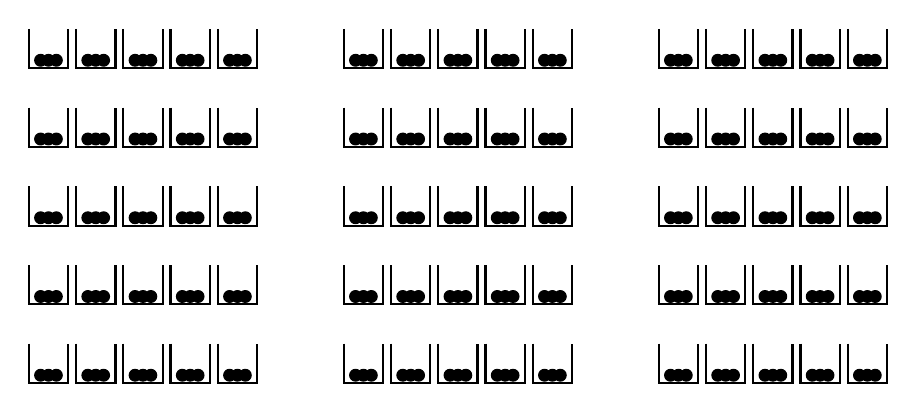
\begin{tikzpicture}[scale=0.5]
\newcommand\lax[3]{
\path[draw,thick,-] (#1-0.5,#2+0.5) -- (#1-0.5,#2-0.5) --
                    (#1+0.5,#2-0.5) -- (#1+0.5,#2+0.5);
\ifthenelse{\equal{#3}{1}}{\draw[fill=black] (#1,#2-0.3) circle (0.15);}{}
\ifthenelse{\equal{#3}{2}}{\draw[fill=black] (#1-0.2,#2-0.3) circle (0.15);}{}
\ifthenelse{\equal{#3}{2}}{\draw[fill=black] (#1+0.2,#2-0.3) circle (0.15);}{}
}
\newcommand\laa[7]{
    \lax{#1}{#2}{#3}
    \lax{#1+1.2}{#2}{#4}
    \lax{#1+2.4}{#2}{#5}
    \lax{#1+3.6}{#2}{#6}
    \lax{#1+4.8}{#2}{#7}
}

\laa{0}{0}{2}{0}{0}{0}{0}
\laa{0}{-2}{1}{1}{0}{0}{0}
\laa{0}{-4}{1}{0}{1}{0}{0}
\laa{0}{-6}{1}{0}{0}{1}{0}
\laa{0}{-8}{1}{0}{0}{0}{1}
\laa{8}{0}{0}{2}{0}{0}{0}
\laa{8}{-2}{0}{1}{1}{0}{0}
\laa{8}{-4}{0}{1}{0}{1}{0}
\laa{8}{-6}{0}{1}{0}{0}{1}
\laa{8}{-8}{0}{0}{2}{0}{0}
\laa{16}{0}{0}{0}{1}{1}{0}
\laa{16}{-2}{0}{0}{1}{0}{1}
\laa{16}{-4}{0}{0}{0}{2}{0}
\laa{16}{-6}{0}{0}{0}{1}{1}
\laa{16}{-8}{0}{0}{0}{0}{2}

\end{tikzpicture}
\end{center}

This process can be represented as a string
that consists of symbols
''o'' and ''$\rightarrow$''.
Initially, we are standing at the leftmost box.
The symbol ''o'' means we place a ball
in the current box, and the symbol
''$\rightarrow$'' means that we move to
the next box right.

Using this notation, each solution is a string
that has $k$ times the symbol ''o'' and
$n-1$ times the symbol ''$\rightarrow$''.
For example, the upper-right solution
corresponds to the string
''$\rightarrow$ $\rightarrow$ o $\rightarrow$ o $\rightarrow$''.
Thus, the number of solutions is
${k+n-1 \choose k}$.

\textit{Case 3}: Each box may contain at most one ball,
and in addition, no two adjacent boxes may both contain a ball.
For example, when $n=5$ and $k=2$,
there are 6 solutions:


\begin{center}
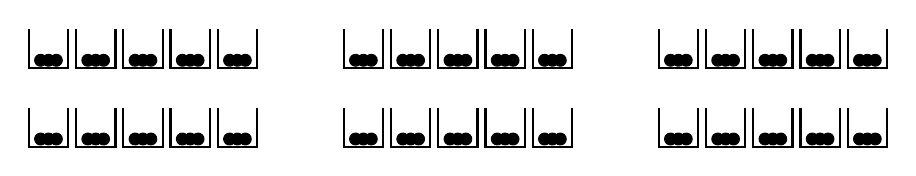
\begin{tikzpicture}[scale=0.5]
\newcommand\lax[3]{
\path[draw,thick,-] (#1-0.5,#2+0.5) -- (#1-0.5,#2-0.5) --
                    (#1+0.5,#2-0.5) -- (#1+0.5,#2+0.5);
\ifthenelse{\equal{#3}{1}}{\draw[fill=black] (#1,#2-0.3) circle (0.15);}{}
\ifthenelse{\equal{#3}{2}}{\draw[fill=black] (#1-0.2,#2-0.3) circle (0.15);}{}
\ifthenelse{\equal{#3}{2}}{\draw[fill=black] (#1+0.2,#2-0.3) circle (0.15);}{}
}
\newcommand\laa[7]{
    \lax{#1}{#2}{#3}
    \lax{#1+1.2}{#2}{#4}
    \lax{#1+2.4}{#2}{#5}
    \lax{#1+3.6}{#2}{#6}
    \lax{#1+4.8}{#2}{#7}
}

\laa{0}{0}{1}{0}{1}{0}{0}
\laa{0}{-2}{1}{0}{0}{1}{0}
\laa{8}{0}{1}{0}{0}{0}{1}
\laa{8}{-2}{0}{1}{0}{1}{0}
\laa{16}{0}{0}{1}{0}{0}{1}
\laa{16}{-2}{0}{0}{1}{0}{1}
\end{tikzpicture}
\end{center}

In this case, we can think that
$k$ balls are initially placed in boxes.
and between each such box there is an empty box.
The remaining task is to choose the
positions for
$n-k-(k-1)=n-2k+1$ empty boxes.
There are $k+1$ positions, so as in case 2,
the number of solutions is
${n-2k+1+k+1-1 \choose n-2k+1} = {n-k+1 \choose n-2k+1}$.

\subsubsection{Multinomial coefficient}

\index{multinomial coefficient}

A generalization for a binomial coefficient is
a \key{multinomial coefficient}

\[ {n \choose k_1,k_2,\ldots,k_m} = \frac{n!}{k_1! k_2! \cdots k_m!}, \]

where $k_1+k_2+\cdots+k_m=n$.
A multinomial coefficient i the number of ways
we can divide $n$ elements into subsets
whose sizes are $k_1,k_2,\ldots,k_m$.
If $m=2$, the formula
corresponds to the binomial coefficient formula.

\section{Catalan numbers}

\index{Catalan number}

A \key{Catalan number} $C_n$ is the
number of valid
parenthesis expressions that consist of
$n$ left parentheses and $n$ right parentheses.

For example, $C_3=5$, because using three
left parentheses and three right parentheses,
we can construct the following parenthesis
expressions:

\begin{itemize}[noitemsep]
\item \texttt{()()()}
\item \texttt{(())()}
\item \texttt{()(())}
\item \texttt{((()))}
\item \texttt{(()())}
\end{itemize}

\subsubsection{Parenthesis expressions}

\index{parenthesis expression}

What is exactly a \emph{valid parenthesis expression}?
The following rules precisely define all
valid parenthesis expressions:

\begin{itemize}
\item The expression \texttt{()} is valid.
\item If a expression $A$ is valid,
then also the expression
\texttt{(}$A$\texttt{)} is valid.
\item If expressions $A$ and $B$ are valid,
then also the expression $AB$ is valid.
\end{itemize}

Another way to characterize valid 
paranthesis expressions is that if
we choose any prefix of the expression,
it has to contain at least as many left
parentheses as right parentheses.
In addition, the complete expression has to
contain an equal number of left and right
parentheses.

\subsubsection{Formula 1}

Catalan numbers can be calculated using the formula
\[ C_n = \sum_{i=0}^{n-1} C_{i} C_{n-i-1}.\]

The sum goes through the ways to divide the
expression into two parts
such that both parts are valid
expressions and the first part is as short as possible
but not empty.
For any $i$, the first part contains $i+1$ pairs
of parentheses, and the number of expressions
is the product of the following values:

\begin{itemize}
\item $C_{i}$: number of ways to construct an expression
using the parentheses in the first part,
not counting the outermost parentheses
\item $C_{n-i-1}$: number of ways to construct an
expression using the parentheses in the second part
\end{itemize}
In addition, the base case is $C_0=1$,
because we can construct an empty parenthesis
expression using zero pairs of parentheses.

\subsubsection{Formula 2}

Catalan numbers can also be calculated
using binomial coefficients:
\[ C_n = \frac{1}{n+1} {2n \choose n}\]
The formula can be explained as follows:

There are a total of ${2n \choose n}$ ways
to construct a (not necessarily valid)
parenthesis expression that contains $n$ left
parentheses and $n$ right parentheses.
Let's calculate the number of such
expressions that are \emph{not} valid.

If a parenthesis expression is not valid,
it has to contain a prefix where the
number of right parentheses exceeds the
number of left parentheses.
The idea is to reverse each parenthesis
that belongs to such a prefix.
For example, the expression
\texttt{())()(} contains a prefix \texttt{())},
and after reversing the prefix,
the expression becomes \texttt{)((()(}.

The resulting expression consists of $n+1$
left parentheses and $n-1$ right parentheses.
The number of such expressions is ${2n \choose n+1}$
that equals the number of non-valid
parenthesis expressions.
Thus the number of valid parenthesis
expressions can be calculated using the formula
\[{2n \choose n}-{2n \choose n+1} = {2n \choose n} - \frac{n}{n+1} {2n \choose n} = \frac{1}{n+1} {2n \choose n}.\]

\subsubsection{Counting trees}

Catalan numbers are also related to rooted trees:

\begin{itemize}
\item there are $C_n$ binary trees of $n$ nodes
\item there are $C_{n-1}$ rooted trees of $n$ nodes
\end{itemize}
\noindent
For example, for $C_3=5$, the binary trees are

\begin{center}
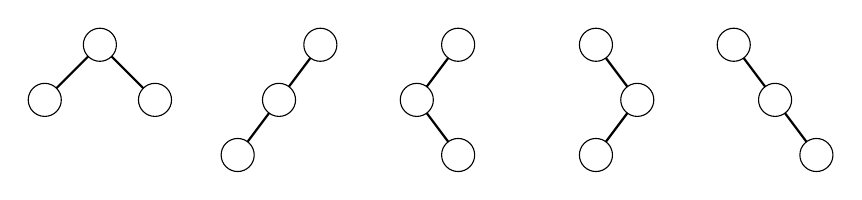
\begin{tikzpicture}[scale=0.7]
\path[draw,thick,-] (0,0) -- (-1,-1);
\path[draw,thick,-] (0,0) -- (1,-1);
\draw[fill=white] (0,0) circle (0.3);
\draw[fill=white] (-1,-1) circle (0.3);
\draw[fill=white] (1,-1) circle (0.3);

\path[draw,thick,-] (4,0) -- (4-0.75,-1) -- (4-1.5,-2);
\draw[fill=white] (4,0) circle (0.3);
\draw[fill=white] (4-0.75,-1) circle (0.3);
\draw[fill=white] (4-1.5,-2) circle (0.3);

\path[draw,thick,-] (6.5,0) -- (6.5-0.75,-1) -- (6.5-0,-2);
\draw[fill=white] (6.5,0) circle (0.3);
\draw[fill=white] (6.5-0.75,-1) circle (0.3);
\draw[fill=white] (6.5-0,-2) circle (0.3);

\path[draw,thick,-] (9,0) -- (9+0.75,-1) -- (9-0,-2);
\draw[fill=white] (9,0) circle (0.3);
\draw[fill=white] (9+0.75,-1) circle (0.3);
\draw[fill=white] (9-0,-2) circle (0.3);

\path[draw,thick,-] (11.5,0) -- (11.5+0.75,-1) -- (11.5+1.5,-2);
\draw[fill=white] (11.5,0) circle (0.3);
\draw[fill=white] (11.5+0.75,-1) circle (0.3);
\draw[fill=white] (11.5+1.5,-2) circle (0.3);
\end{tikzpicture}
\end{center}
and the rooted trees are
\begin{center}
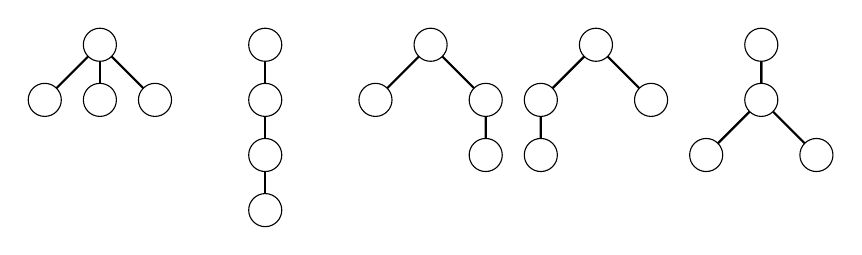
\begin{tikzpicture}[scale=0.7]
\path[draw,thick,-] (0,0) -- (-1,-1);
\path[draw,thick,-] (0,0) -- (0,-1);
\path[draw,thick,-] (0,0) -- (1,-1);
\draw[fill=white] (0,0) circle (0.3);
\draw[fill=white] (-1,-1) circle (0.3);
\draw[fill=white] (0,-1) circle (0.3);
\draw[fill=white] (1,-1) circle (0.3);

\path[draw,thick,-] (3,0) -- (3,-1) -- (3,-2) -- (3,-3);
\draw[fill=white] (3,0) circle (0.3);
\draw[fill=white] (3,-1) circle (0.3);
\draw[fill=white] (3,-2) circle (0.3);
\draw[fill=white] (3,-3) circle (0.3);

\path[draw,thick,-] (6+0,0) -- (6-1,-1);
\path[draw,thick,-] (6+0,0) -- (6+1,-1) -- (6+1,-2);
\draw[fill=white] (6+0,0) circle (0.3);
\draw[fill=white] (6-1,-1) circle (0.3);
\draw[fill=white] (6+1,-1) circle (0.3);
\draw[fill=white] (6+1,-2) circle (0.3);

\path[draw,thick,-] (9+0,0) -- (9+1,-1);
\path[draw,thick,-] (9+0,0) -- (9-1,-1) -- (9-1,-2);
\draw[fill=white] (9+0,0) circle (0.3);
\draw[fill=white] (9+1,-1) circle (0.3);
\draw[fill=white] (9-1,-1) circle (0.3);
\draw[fill=white] (9-1,-2) circle (0.3);

\path[draw,thick,-] (12+0,0) -- (12+0,-1) -- (12-1,-2);
\path[draw,thick,-] (12+0,0) -- (12+0,-1) -- (12+1,-2);
\draw[fill=white] (12+0,0) circle (0.3);
\draw[fill=white] (12+0,-1) circle (0.3);
\draw[fill=white] (12-1,-2) circle (0.3);
\draw[fill=white] (12+1,-2) circle (0.3);

\end{tikzpicture}
\end{center}

\section{Inclusion-exclusion}

\index{inclusion-exclusion}

\key{Inclusion-exclusion} is a technique
that can be used for counting the size
of a union of sets when the sizes of
the intersections are known, and vice versa.
A simple example of the technique is the formula
\[ |A \cup B| = |A| + |B| - |A \cap B|,\]
where $A$ and $B$ are sets and $|X|$
is the size of a set $X$.
The formula can be illustrated as follows:

\begin{center}
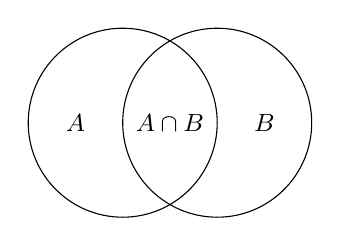
\begin{tikzpicture}[scale=0.8]

\draw (0,0) circle (1.5);
\draw (1.5,0) circle (1.5);

\node at (-0.75,0) {\small $A$};
\node at (2.25,0) {\small $B$};
\node at (0.75,0) {\small $A \cap B$};

\end{tikzpicture}
\end{center}

In the above example, our goal is to calculate
the size of the union $A \cup B$
that corresponds to the area of the region
that is inside at least one circle.
The picture shows that we can calculate
the area of $A \cup B$ by first summing the
areas of $A$ and $B$, and then subtracting
the area of $A \cap B$.

The same idea can be applied, when the number
of sets is larger.
When there are three sets, the formula becomes
\[ |A \cup B \cup C| = |A| + |B| + |C| - |A \cap B|  - |A \cap C|  - |B \cap C| + |A \cap B \cap C| \]
and the corresponding picture is

\begin{center}
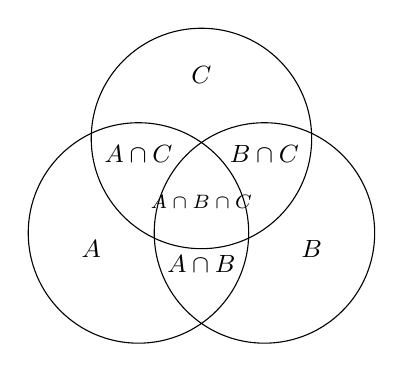
\begin{tikzpicture}[scale=0.8]

\draw (0,0) circle (1.75);
\draw (2,0) circle (1.75);
\draw (1,1.5) circle (1.75);

\node at (-0.75,-0.25) {\small $A$};
\node at (2.75,-0.25) {\small $B$};
\node at (1,2.5) {\small $C$};
\node at (1,-0.5) {\small $A \cap B$};
\node at (0,1.25) {\small $A \cap C$};
\node at (2,1.25) {\small $B \cap C$};
\node at (1,0.5) {\scriptsize $A \cap B \cap C$};

\end{tikzpicture}
\end{center}

In the general case, the size of the 
union $X_1 \cup X_2 \cup \cdots \cup X_n$
can be calculated by going through all ways to
construct an intersection for a collection of
sets $X_1,X_2,\ldots,X_n$.
If the intersection contains an odd number of sets,
its size will be added to the answer,
and otherwise subtracted from the answer.

Note that similar formulas also work when counting
the size of an intersection from the sizes of
unions. For example,
\[ |A \cap B| = |A| + |B| - |A \cup B|\]
and
\[ |A \cap B \cap C| = |A| + |B| + |C| - |A \cup B|  - |A \cup C|  - |B \cup C| + |A \cup B \cup C| .\]

\subsubsection{Derangements}

\index{derangement}

As an example, let's count the number of \key{derangements}
of numbers $\{1,2,\ldots,n\}$, i.e., permutations
where no element remains in its original place.
For example, when $n=3$, there are
two possible derangements: $(2,3,1)$ ja $(3,1,2)$.

One approach for the problem is to use
inclusion-exclusion.
Let $X_k$ be the set of permutations
that contain the number $k$ at index $k$.
For example, when $n=3$, the sets are as follows:
\[
\begin{array}{lcl}
X_1 & = & \{(1,2,3),(1,3,2)\} \\
X_2 & = & \{(1,2,3),(3,2,1)\} \\
X_3 & = & \{(1,2,3),(2,1,3)\} \\
\end{array}
\]
Using these sets the number of derangements is
\[ n! - |X_1 \cup X_2 \cup \cdots \cup X_n|, \]
so it suffices to calculate the size of the union.
Using inclusion-exclusion, this reduces to
calculating sizes of intersections which can be
done efficiently.
For example, when $n=3$, the size of
$|X_1 \cup X_2 \cup X_3|$ is
\[
\begin{array}{lcl}
 & & |X_1| + |X_2| + |X_3| - |X_1 \cap X_2|  - |X_1 \cap X_3|  - |X_2 \cap X_3| + |X_1 \cap X_2 \cap X_3| \\
 & = & 2+2+2-1-1-1+1 \\
 & = & 4, \\
\end{array}
\]
so the number of solutions is $3!-4=2$.

It turns out that there is also another way for
solving the problem without inclusion-exclusion.
Let $f(n)$ denote the number of derangements
for $\{1,2,\ldots,n\}$. We can use the following
recursive formula:

\begin{equation*}
    f(n) = \begin{cases}
               0               & n = 1\\
               1               & n = 2\\
               (n-1)(f(n-2) + f(n-1)) & n>2 \\
           \end{cases}
\end{equation*}

The formula can be derived by going through
the possibilities how the number 1 changes
in the derangement.
There are $n-1$ ways to choose a number $x$
that will replace the number 1.
In each such choice, there are two options:

\textit{Option 1:} We also replace the number $x$
by the number 1.
After this, the remaining task is to construct
a derangement for $n-2$ numbers.

\textit{Option 2:} We replace the number $x$
by some other number than 1.
Now we should construct a derangement
for $n-1$ numbers, because we can't replace
the number $x$ with number $1$, and all other
numbers should be changed.

\section{Burnsiden lemma}

\index{Burnsiden lemma@Burnsiden lemma}

\key{Burnsiden lemma} laskee yhdistelmien määrän niin,
että symmetrisistä yhdistelmistä lasketaan
mukaan vain yksi edustaja.
Burnsiden lemman mukaan yhdistelmien määrä on
\[\sum_{k=1}^n \frac{c(k)}{n},\]
missä yhdistelmän asentoa voi muuttaa $n$ tavalla
ja $c(k)$ on niiden yhdistelmien määrä,
jotka pysyvät ennallaan, kun asentoa
muutetaan tavalla $k$.

Lasketaan esimerkkinä, montako
erilaista tapaa on
muodostaa $n$ helmen helminauha,
kun kunkin helmen värin tulee olla
väliltä $1,2,\ldots,m$.
Kaksi helminauhaa ovat symmetriset,
jos ne voi saada näyttämään samalta pyörittämällä.
Esimerkiksi helminauhan
\begin{center}
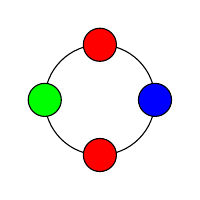
\begin{tikzpicture}[scale=0.7]
\draw[fill=white] (0,0) circle (1);
\draw[fill=red] (0,1) circle (0.3);
\draw[fill=blue] (1,0) circle (0.3);
\draw[fill=red] (0,-1) circle (0.3);
\draw[fill=green] (-1,0) circle (0.3);
\end{tikzpicture}
\end{center}
kanssa symmetriset helminauhat ovat seuraavat:
\begin{center}
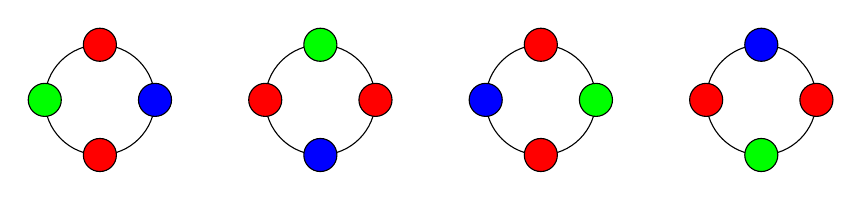
\begin{tikzpicture}[scale=0.7]
\draw[fill=white] (0,0) circle (1);
\draw[fill=red] (0,1) circle (0.3);
\draw[fill=blue] (1,0) circle (0.3);
\draw[fill=red] (0,-1) circle (0.3);
\draw[fill=green] (-1,0) circle (0.3);

\draw[fill=white] (4,0) circle (1);
\draw[fill=green] (4+0,1) circle (0.3);
\draw[fill=red] (4+1,0) circle (0.3);
\draw[fill=blue] (4+0,-1) circle (0.3);
\draw[fill=red] (4+-1,0) circle (0.3);

\draw[fill=white] (8,0) circle (1);
\draw[fill=red] (8+0,1) circle (0.3);
\draw[fill=green] (8+1,0) circle (0.3);
\draw[fill=red] (8+0,-1) circle (0.3);
\draw[fill=blue] (8+-1,0) circle (0.3);

\draw[fill=white] (12,0) circle (1);
\draw[fill=blue] (12+0,1) circle (0.3);
\draw[fill=red] (12+1,0) circle (0.3);
\draw[fill=green] (12+0,-1) circle (0.3);
\draw[fill=red] (12+-1,0) circle (0.3);
\end{tikzpicture}
\end{center}
Tapoja muuttaa asentoa on $n$,
koska helminauhaa voi pyörittää $0,1,\ldots,n-1$
askelta myötäpäivään.
Jos helminauhaa pyörittää 0 askelta,
kaikki $m^n$ väritystä säilyvät ennallaan.
Jos taas helminauhaa pyörittää 1 askeleen,
vain $m$ yksiväristä helminauhaa säilyy ennallaan.

Yleisemmin kun helminauhaa pyörittää $k$ askelta,
ennallaan säilyvien yhdistelmien määrä on
\[m^{\textrm{syt}(k,n)},\]
missä $\textrm{syt}(k,n)$ on lukujen $k$ ja $n$
suurin yhteinen tekijä.
Tämä johtuu siitä, että $\textrm{syt}(k,n)$-kokoiset
pätkät helmiä siirtyvät toistensa paikoille
$k$ askelta eteenpäin.
Niinpä helminauhojen määrä on
Burnsiden lemman mukaan
\[\sum_{i=0}^{n-1} \frac{m^{\textrm{syt}(i,n)}}{n}. \]
Esimerkiksi kun helminauhan pituus on 4
ja värejä on 3, helminauhoja on
\[\frac{3^4+3+3^2+3}{4} = 24. \]

\section{Cayleyn kaava}

\index{Cayleyn kaava@Cayleyn kaava}

\key{Cayleyn kaavan} mukaan $n$ solmusta voi
muodostaa $n^{n-2}$ numeroitua puuta.
Puun solmut on numeroitu $1,2,\ldots,n$,
ja kaksi puuta ovat erilaiset,
jos niiden rakenne on erilainen
tai niissä on eri numerointi.

\begin{samepage}
\noindent
Esimerkiksi kun $n=4$, numeroitujen puiden määrä on $4^{4-2}=16$:

\begin{center}
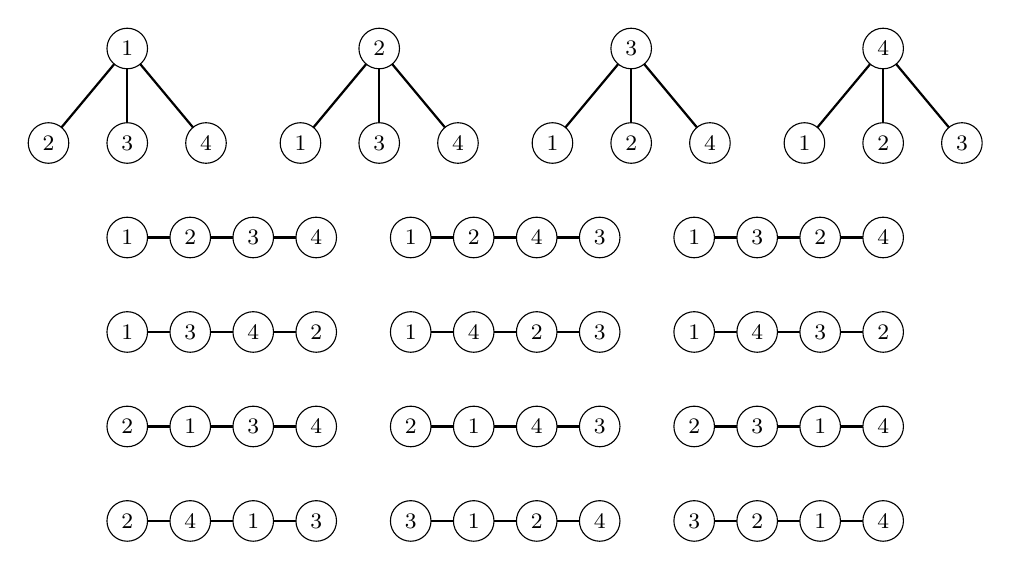
\begin{tikzpicture}[scale=0.8]
\footnotesize

\newcommand\puua[6]{
\path[draw,thick,-] (#1,#2) -- (#1-1.25,#2-1.5);
\path[draw,thick,-] (#1,#2) -- (#1,#2-1.5);
\path[draw,thick,-] (#1,#2) -- (#1+1.25,#2-1.5);
\node[draw, circle, fill=white] at (#1,#2) {#3};
\node[draw, circle, fill=white] at (#1-1.25,#2-1.5) {#4};
\node[draw, circle, fill=white] at (#1,#2-1.5) {#5};
\node[draw, circle, fill=white] at (#1+1.25,#2-1.5) {#6};
}
\newcommand\puub[6]{
\path[draw,thick,-] (#1,#2) -- (#1+1,#2);
\path[draw,thick,-] (#1+1,#2) -- (#1+2,#2);
\path[draw,thick,-] (#1+2,#2) -- (#1+3,#2);
\node[draw, circle, fill=white] at (#1,#2) {#3};
\node[draw, circle, fill=white] at (#1+1,#2) {#4};
\node[draw, circle, fill=white] at (#1+2,#2) {#5};
\node[draw, circle, fill=white] at (#1+3,#2) {#6};
}

\puua{0}{0}{1}{2}{3}{4}
\puua{4}{0}{2}{1}{3}{4}
\puua{8}{0}{3}{1}{2}{4}
\puua{12}{0}{4}{1}{2}{3}

\puub{0}{-3}{1}{2}{3}{4}
\puub{4.5}{-3}{1}{2}{4}{3}
\puub{9}{-3}{1}{3}{2}{4}
\puub{0}{-4.5}{1}{3}{4}{2}
\puub{4.5}{-4.5}{1}{4}{2}{3}
\puub{9}{-4.5}{1}{4}{3}{2}
\puub{0}{-6}{2}{1}{3}{4}
\puub{4.5}{-6}{2}{1}{4}{3}
\puub{9}{-6}{2}{3}{1}{4}
\puub{0}{-7.5}{2}{4}{1}{3}
\puub{4.5}{-7.5}{3}{1}{2}{4}
\puub{9}{-7.5}{3}{2}{1}{4}
\end{tikzpicture}
\end{center}
\end{samepage}

Seuraavaksi näemme, miten Cayleyn kaavan
voi perustella samastamalla numeroidut puut
Prüfer-koodeihin.

\subsubsection{Prüfer-koodi}

\index{Prüfer-koodi}

\key{Prüfer-koodi} on $n-2$ luvun jono,
joka kuvaa numeroidun puun rakenteen.
Koodi muodostuu poistamalla puusta
joka askeleella lehden, jonka numero on pienin,
ja lisäämällä lehden vieressä olevan solmun
numeron koodiin.

Esimerkiksi puun
\begin{center}
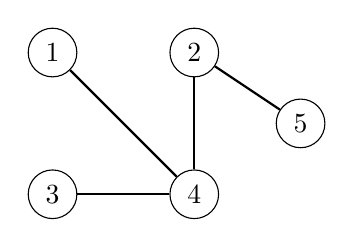
\begin{tikzpicture}[scale=0.9]
\node[draw, circle] (1) at (2,3) {$1$};
\node[draw, circle] (2) at (4,3) {$2$};
\node[draw, circle] (3) at (2,1) {$3$};
\node[draw, circle] (4) at (4,1) {$4$};
\node[draw, circle] (5) at (5.5,2) {$5$};

%\path[draw,thick,-] (1) -- (2);
%\path[draw,thick,-] (1) -- (3);
\path[draw,thick,-] (1) -- (4);
\path[draw,thick,-] (3) -- (4);
\path[draw,thick,-] (2) -- (4);
\path[draw,thick,-] (2) -- (5);
%\path[draw,thick,-] (4) -- (5);
\end{tikzpicture}
\end{center}
Prüfer-koodi on $[4,4,2]$,
koska puusta poistetaan ensin solmu 1,
sitten solmu 3 ja lopuksi solmu 5.

Jokaiselle puulle voidaan laskea
Prüfer-koodi, minkä lisäksi
Prüfer-koodista pystyy palauttamaan
yksikäsitteisesti alkuperäisen puun.
Niinpä numeroituja puita on yhtä monta
kuin Prüfer-koodeja eli $n^{n-2}$.

